\documentclass[conference]{IEEEtran}
\IEEEoverridecommandlockouts
% The preceding line is only needed to identify funding in the first footnote. If that is unneeded, please comment it out.
\usepackage{cite}
\usepackage{amsmath,amssymb,amsfonts}
\usepackage{algorithmic}
\usepackage[dvipdfmx]{graphicx}
\usepackage[dvipdfmx]{color}
\usepackage{textcomp}
\usepackage{xcolor}
\usepackage{comment}
\usepackage{listings}

\lstset{%
  language={Java},
  basicstyle={\scriptsize},%
  identifierstyle={\scriptsize},%
  commentstyle={\scriptsize\itshape},%
  keywordstyle={\color{red}\scriptsize\bfseries},  
  ndkeywordstyle={\scriptsize},%
  stringstyle={\scriptsize\ttfamily},
  frame={tb},
  breaklines=true,
  columns=[l]{fullflexible},%
  numbers=left,%
  xrightmargin=0cm,%
  xleftmargin=0.3cm,%
  numberstyle={\scriptsize},%
  stepnumber=1,
  numbersep=0.2cm,%
  lineskip=-0.1ex%
}


\def\BibTeX{{\rm B\kern-.05em{\sc i\kern-.025em b}\kern-.08em
    T\kern-.1667em\lower.7ex\hbox{E}\kern-.125emX}}
\begin{document}

\title{SuiteRec: Automatic Test Suite Recommendation System based on Code Clone Detection\\
%{\footnotesize \textsuperscript{*}Note: Sub-titles are not captured in Xplore and
%should not be used}
%\thanks{Identify applicable funding agency here. If none, delete this.}
}


%%%%%
\author{\IEEEauthorblockN{Ryosuke Kurachi\IEEEauthorrefmark{1},  Eunjong Choi\IEEEauthorrefmark{2}, Dongsun Kim\IEEEauthorrefmark{3},Keichi Takahashi\IEEEauthorrefmark{1},  and Hajimu Iida\IEEEauthorrefmark{1}}
\IEEEauthorblockA{\IEEEauthorrefmark{1}Nara Institute of Science and Technology, Japan, \{kurachi.ryosuke.kp0, keichi\}@is.naist.jp, iida@itc.naist.jp}
\IEEEauthorblockA{\IEEEauthorrefmark{2}Kyoto Institute of Technology, Japan, echoi@kit.ac.jp\\}
\IEEEauthorblockA{\IEEEauthorrefmark{3}FuriosaAI, South Korea, darkrsw@furiosa.ai\\}
}
\maketitle

\begin{abstract}
%Software testing is vital to ensure the quality of software. In previous studies, various techniques to automatically generate test codes have been proposed to reduce development costs. However, automatically generated tests tend to ignore the development process and intention behind the target code, and therefore generally considered to be less readable and maintainable. This places a question mark over their practical value. To solve this problem, we propose SuiteRec, a recommendation tool to find existing high-quality test codes from OSS projects. The basic idea behind SuiteRec is that test codes can be reused between clone pairs. SuiteRec finds code clones of the input code from OSS projects and recommends test suites corresponding to the clones. The recommended test suites are sorted by their quality and presented to the developer. Furthermore, test smells, which indicate bad implementation of test codes, are shown for each test suite. In the evaluation, we asked subjects to develop test codes with and without using SuiteRec and compared the developed test codes. We show that (1) SuiteRec improves code coverage when developing test codes for target codes with many conditional branches, (2) test codes developd using SuiteRec have higher quality and less test smells, and (3) developers feel that it is easier to develop test codes, and they are more confident in the resulting test codes when using SuiteRec.

Automatically generated tests generally ignore the development process and intention behind the target code, and therefore generally tend to be less readable and maintainable. Reusing existing tests might solve this problem. To this end, we developed SuiteRec, a system that recommends high-quality reusable test suites based on code clone detection. Given a java Method, SuiteRec detects its code clones from OSS projects and then shows test suites of the cloned clones. It provides the ranking that shows the test suites based on the test smells and similarity between the input code and the cloned code. We evaluate SuiteRec with a human study of 10 student developers. The results indicate that SuiteRec successfully recommends high-quality reusable test suites.
\begin{comment}
ソフトウェアの品質確保の要と言えるソフトウェアテストを支援することは重要です.これまでに,テスト作成コストを削減するために様々な自動生成技術が提案されてきました.しかし,自動生成されたテストコードはテスト対象コードの作成経緯や意図に基づいて生成されていないという性質から後のメンテナンス活動を困難にさせる課題があり,これは自動生成技術の実用的な利用の価値に疑問を提示させます.本研究では,この課題を解決するために,OSSに上に存在する既存の品質の高いテストコード推薦するツールSuiteRecを紹介します.SuiteRecは,類似コード検索ツールを用いてクローンペア間でのテスト再利用を考えます.入力コードに対して類似コードを検出し,その類似コードに対応するテストスイートを開発者に推薦します.さらに,テストコードの良くない実装を表すメトリクスであるテストスメルを開発者に提示し,より品質の高いテストスイートを推薦できるように推薦順位がランキングされています.提案ツールの評価では,被験者によってSuiteRecの使用した場合とそうでない場合でテストコードの作成してもらい,テスト作成をどの程度支援できるかを定量的および定性的に評価しました.その結果,(1) 条件分岐が多いプログラムのテストコードを作成する際にコードカバレッジの向上に効果的であること,(2) SuiteRecを使用した場合,テストコードの作成に時間がかかること,(3) SuiteRecを使用して作成したテストコードは検出されたテストスメルの数が少なく品質が高いこと,(4) SuiteRecを使用してテストコードを作成した場合は使用しなかった場合と比べて開発者は,自身で作成したテストコードに自信が持てることが分かった.
\end{comment}
%This document is a model and instructions for \LaTeX.
%This and the IEEEtran.cls file define the components of your paper [title, text, heads, etc.]. *CRITICAL: Do Not Use Symbols, Special Characters, Footnotes, 
%or Math in Paper Title or Abstract.
\end{abstract}

\begin{IEEEkeywords}
 clone detection, recommendation system, software testing, unit test 
\end{IEEEkeywords}

\section{Introduction}
In recent years, the requirements for software have become more sophisticated and diversified, while the demands from users for ensuring software quality and reducing costs have also increased. Among them, it is important to support software testing, which accounts for a large percentage of the total software development cost\cite{b20}. However, at present, most of unit tests are developed manually, and if you try to develop many tests, the cost will increase proportionally. Against this background, various automation technologies have been proposed to ensure software quality and achieve cost reduction\cite{b3},\cite{b16},\cite{b17},\cite{b18},\cite{b19}. 

For example, EvoSuite\cite{b3} is the most advanced tool for automatic unit test generation. EvoSuite statically analyzes the target code and expresses the program as symbolic values. Then, conditions that pass the control path of the target code are collected, and concrete values that satisfy the conditions are generated. By automatically generating tests, developers can save creation time and increase code coverage. However, the automatically generated test code is low readability and is not trusted by developers because it is not based on the development process and intention behind the target code, which makes later maintenance activities difficult\cite{b13},\cite{b14},\cite{b15}. Every time a test fails, the developer has to identify the cause of the failure in the production code or determine whether the test itself needs to be updated. Previous studies have reported that automatically generated tests are harder to read outweigh the time-savings gained by their automated generation, and render them more of a hindrance than a help for software maintenance\cite{b1}.

In this paper,  to solve this problem, we propose SuiteRec, a recommendation tool to find existing high-quality test codes from OSS projects. 

The contributions from SuiteRec are shown below:

\noindent
$\bullet$ \textbf{Test suite recommendation method.} We proposed test suites search method from OSS projects. The basic idea behind SuiteRec is that test codes can be reused between clone pairs. SuiteRec finds code clones of the input code from OSS projects and recommends test suites corresponding to the clones. The recommended test suites are sorted by their quality and presented to the developer. Furthermore, test smells, which indicate bad implementation of test codes, are shown for each test suite.

\noindent
$\bullet$ \textbf{Quantitative and qualitative evaluation of SuiteRec.} We asked subjects to develop test code with and without SuiteRec, and compared the developed tests to evaluate how much test development can be supported. As a result, using SuiteRec is effective in increasing code coverage when developing test code for target code with many conditional branchesand test codes developed using SuiteRec have higher quality and less test smells. In addition, qualitative evaluation by questionnaire after the experiment showed that subjects feel that it is easier to develop test codes, and they are more confident in the resulting test codes when using SuiteRec.


\begin{comment}
提案ツールの評価では,被験者によってSuiteRecの使用した場合とそうでない場合でテストコードの作成してもらい,テスト作成をどの程度支援できるかを定量的および定性的に評価した.その結果,提案ツールの利用は分岐が多く複雑なプログラムのテストスイートを作成する際に,コードカバレッジを向上させることができることや,ツールを使用して作成テストコードの品質が高いことが分かった.また,定性的な評価として実験後にアンケートを実施し,推薦ツールを使った場合多くの被験者は自分の作成したテストコードに自信が持てることが分かった.
\end{comment}


\section{BACKGROUND AND RELETED WORK}

\begin{figure*}[t]
\begin{center}
  \begin{tabular}{c}

    % 1枚目の画像
    \begin{minipage}{0.5\hsize}
      \begin{center}
\begin{lstlisting}
public class ConvertString {
    public static String convertSnakeCase(String name) {
        if (name == null) throw new NullPointerException();
        String method = name;
        Pattern p = Pattern.compile("([A-Z])");
        for (;;) {
            Matcher m = p.matcher(name);
            if (!m.find()) break;
            method = m.replaceFirst("_" + m.group(1).toLowerCase());
        }
        return method.replaceFirst("^_", "");
    }
}
\end{lstlisting}
{\scriptsize (a) Target Code fragment}
\end{center}
\end{minipage}

    % 2枚目の画像
    \begin{minipage}{0.5\hsize}
      \begin{center}
\begin{lstlisting}
public class StringUtils {
    public String toSnakeCase(String text) {
        if (text == null) throw new NullPointerException();
        String snake = text;
        Pattern p = Pattern.compile("([A-Z])");
        for (;;) {
            Matcher m = p.matcher(snake);
            if (!m.find()) break;
            snake = m.replaceFirst("_" + m.group(1).toLowerCase());
        }
        return snake.replaceFirst("^_", "");
    }
}
\end{lstlisting}
{\scriptsize (b) Similar Code fragment}
      \end{center}
    \end{minipage}
  \end{tabular}
  \end{center}
\end{figure*}

\begin{figure}[htbp]
\begin{center}
\begin{lstlisting}
 public class StringUtilsTest {
     @Test(expected = NullPointerException.class)
     public void expectedExceptionfor_null() throws Exception {
    	 StringUtils sut = new StringUtils();
    	 sut.toSnakeCase(null);
     }
    
     @Test
     public void returnSnakeCasefor_HelloWorld() throws Exception {
     	 StringUtils sut = new StringUtils();
    	 String expected = "hello_world";
    	 String actual = sut.toSnakeCase("HelloWorld");
         assertThat(actual, is(expected));
     }
     ...
 }
\end{lstlisting}
{\scriptsize (c) Test suite for similar code fragments}
\end{center}
\end{figure}

In the unit test execution task, the software is run, and it is confirmed whether the software behaves as expected in each test case. In order to reduce the cost of the test process, in test execution tasks, the use of automatic test execution tools such as JUnit is advancing in the industry for unit tests. However, test design tasks are still often performed manually, and the practical application and popularization of automation technology is expected.

Test cases developed by unit test design tasks consist of test procedures, test input values, and expected test results. The test input value is given to the software under test according to the test procedure, and the output result is compared with the expected test result. If they match, the test passes, otherwise it fails. In unit test design tasks, test input values are often developd using test case creation techniques such as equivalence partitioning and boundary analysis, but there are many variations to verify that the software works as required. You need to develop test input values for.

\begin{comment}
\textbf {Test case generation.} Existing research \cite {b12} demonstrates that existing test cases can be reused, automatically generated, or reapplied to save significant time and money in the software development testing process. It shows. There are five main test generation techniques: random test (RT), symbol execution (SE), search base test (SBST), model base (MBT), and combination test. SE is further divided into static symbol execution (SSE) and dynamic symbol execution (DSE).

RT is a test method that gives random input to the software. Random tests that run randomly and uniformly are suitable for automation, but the efficiency per test case is extremely poor in terms of improving code coverage and bug detection.

SE analyzes the target code statically, expresses the program as a symbolic value, extracts the conditions corresponding to each path in the code, and collects the conditions that the input values that pass through the path must satisfy. For each path, the conditions are solved using a constraint solver such as the SMT solver [5], and the obtained concrete value is used as the test input value.

SBST is a generic name for technologies that generate test suites that satisfy the requirements to be achieved using a heuristic search algorithm based on an evaluation function designed to quantitatively evaluate the degree of achievement for the requirements to be achieved.

MBT is a general term for technologies that generate test suites based on models. The model describes the target in some form. The model for requirements analysis and design may be used, or the model may be developed for testing.

CT is a method of generating combinations of values assigned to parameters as test cases in order to effectively find defects caused by interaction between parameters.
\end{comment}

% \textbf{Unit testing. }単体テストの実行タスクでは,ソフトウェアを動作させ,それぞれのテストケースにおいてソフトウェアが期待通りの振る舞いをするかを確認する.テスト工程のコスト削減のため,テスト実行タスクにおいて,単体テストではJUnitなどのテスト自動実行ツールの利用が産業界で進んでいる.しかし,テスト設計タスクは未だ手動で行うことが多く,自動化技術の実用化および普及が期待されている.

% 単体テスト設計タスクで作成されるテストケースは,テスト手順,テスト入力値,テスト期待結果から構成される.テスト手順に従ってテスト対象のソフトウェアにテスト入力値を与え,その出力結果をテスト期待結果と比較する.これが一致していればテストは合格となり,一致しなければ不合格となる.単体テスト設計タスクにおいては,多くの場合同値分割法,境界地分析法などのテストケース作成技法を用いてテスト入力値を作成するが,ソフトウェアの要求通りに動作するかを確認するために多くのバリエーションのテスト入力値を作成する必要がある.

% \textbf{Test case generation. }既存の研究\cite{b12}は,既存のテストケースを再利用,自動生成,または再適用できることによって,ソフトウェア開発のテスト工程における時間とコストを大幅に節約できることを示している.テスト生成技術は,主にランダムテスト(RT),記号実行(SE),サーチベーステスト(SBST),モデルベース(MBT),組み合わせテストの5つに分類できる.SEはさらに静的記号実行(SSE)と動的記号実行(DSE)に分けられる.

% RTとは,ソフトウェアにランダムな入力を与えるテスト手法である.無造作・均一にテストを実行するランダムテストは自動化に適しているが,コードカバレッジ率向上,バグ検出の観点において,テストケース1件当たりの効率は著しく悪い.

% SEは対象コードを静的解析してプログラムを記号値で表現し,コード上のそれぞれのパスに対応する条件を抽出し,パスごとにパスを通るような入力値が満たすべき条件を集める.そして,パスごとにその条件をSMTソルバ[5]などの制約ソルバを用いて解き,得られた具体値をテスト入力値とする.

% SBSTは,達成したい要件に対する達成度合いを定量的に評価できるように設計した評価関数に基づいて,ヒューリスティック探索アルゴリズムを用いて達成したい要件を満足するテストスイートを生成する技術の総称である.

% MBTはモデルに基づいてテストスイートを生成する技術の総称である.モデルは何らかの形でテスト対象を記述したものであり,要求分析や設計のためのモデルを活用することもあれば,テストのためにモデルを作成することもある.

% CTは,パラメータ間の相互作用に起因する不具合を効果的に発見するためにテストケースとしてパラメータに割り当てる値の組み合わせを生成する手法である.

\textbf{Test Smell.} The importance of having well-designed test code was initially put forward by Beck\cite{b4}. Beck argued that test cases respecting good design principles are desirable since these test cases are easier to comprehend, maintain, and can be successfully exploited to diagnose problems in the production code. Inspired by these arguments, van Deursen et al.\cite{b7} coined the them test smells and defined the first catalog of 11 poor design choices to write tests, together with refactoring operations aimed at removing them. Such a catalog has been then extended more recently by practitioners, such as Meszaros\cite{b6} who defined 18 new test smells. As reported by recent studies, their presence might not only negatively affect the comprehension of test suites but can also lead to test cases being less effective in finding bugs in production code\cite{b8}.

\section{SuiteRec}
%\textsf{SuiteRec} takes a code fragment from the developer and searches in exsiting OSS projects to identify test suites that are correspond to the developer’s input. Furthermore, test smells in test suites are detected, and test suites are ranked in descending order of quality.
\textsf{SuiteRec} detects cloned code of given input and then identifies test suites of that are correspond to the developer’s input. Furthermore, test smells in test suites are detected, and test suites are ranked in descending order of quality.


Figure \ref{fig1} shows the flow until test suites are recommended by \textsf{SuiteRec} . The recommendation method mainly consists of the following four steps.


\begin{figure}[htbp]
\centerline{\includegraphics[width=8.5cm]{SuiteRec-outline.pdf}}
\caption{Overview of SuiteRec}
\label{fig1}
\end{figure}

\begin{enumerate}
\renewcommand{\labelenumi}{(\arabic{enumi})}
\item When SuiteRec receives a input code, it searches the corresponding similar code fragments from the Source Code Database using a existing clone detection tool.
\item Detected similar code fragments, SuiteRec searches test suites corresponding to similar code fragments from the Test  Code Database.
\item SuiteRec detects test smells in the test suites collected by the previous step using a test smell detection tool.
\item As the final step, SuiteRec ranks recommended test suites based on similarity and number of test smells.
\end{enumerate}


\subsection{Code Clone Detection}
At first, SuiteRec detects code clones of the input code. To detect In this study, NICAD\cite{b2} was adopted as a code clone detection tool. NICAD detects clone pairs by converting the layout of code fragments and comparing code fragments line by line. By taking this approach, NICAD has realized clone pair detection with high accuracy and high recall. SuiteRec searches for projects that include input code by using NICAD, and outputs similar codes corresponding to the input codes in the detected clone pairs.

The Source Code Database in Figure \ref{fig1} contains only target code fragments of the Github projects with test codes. Specifically, we selected projects that had  test folders in the projects and adopted the JUnit testing framework. 

NICAD has a project size limit that can be searched at once. In oerder to shorten the search time, large-scale projects were divided, small-scale projects were integrated, and multiple search processes were run in parallel, making it possible to search for similar code fragments in real time. The detection setting is implemented in the SuiteRec as a standard setting of NICAD.

\begin{table*}[t]
\caption{Subject Test Smells}
\label{smells}
\begin{tabular}{|l|p{14.5cm}|}
\hline
\textbf{Name}                   & \textbf{Description}                                                                                                       \\ \hline
\textbf{Assetion Roulette}        & Occurs when a test method has multiple assertions. Multiple assertion statements in a test method without a descriptive message impacts readability/understandability/maintainability as it’s not possible to understand the reason for the failure of the test.  \\ \hline
\textbf{Conditional Test Logic} & Test methods need to be simple and execute all statements in the production method. Conditional code with in a test method negatively impacts the ease of comprehension by developers.\\ \hline
\textbf{Default Test}            & Test code in which the test class or test method name is the default in test code using a testing framework such as JUnit. It is necessary to change the name appropriately to improve the readability of the code.                                                                                                      \\ \hline
\textbf{Eager Test }             & Occurs when a test method invokes several methods of the production object. This smell results in difficulties in test comprehension and maintenance. \\ \hline
\textbf{Exception Handling}      & This smell occurs when a test method explicitly a passing or failing of a test method is dependent on the production method throwing an exception. Developers should utilize JUnit's exception handling to automatically pass/fail the test instead of writing custom exception handling code or throwing an exception. \\ \hline
\textbf{Mystery Guest}          & Occurs when a test method utilizes external resources (e.g. files, database, etc.). Use of external resources in test methods will result in stability and performance issues. Developers should use mock objects in place of external resources. \\ \hline
\end{tabular}
\end{table*}

\subsection{Test Code Detection}
In order to search for test suites corresponding to similar code fragments, the target code is linked with test code fragments. In this research, the following two steps are taken in order to precisely link the target code with test code fragments.

\begin{figure}[htbp]
\centerline{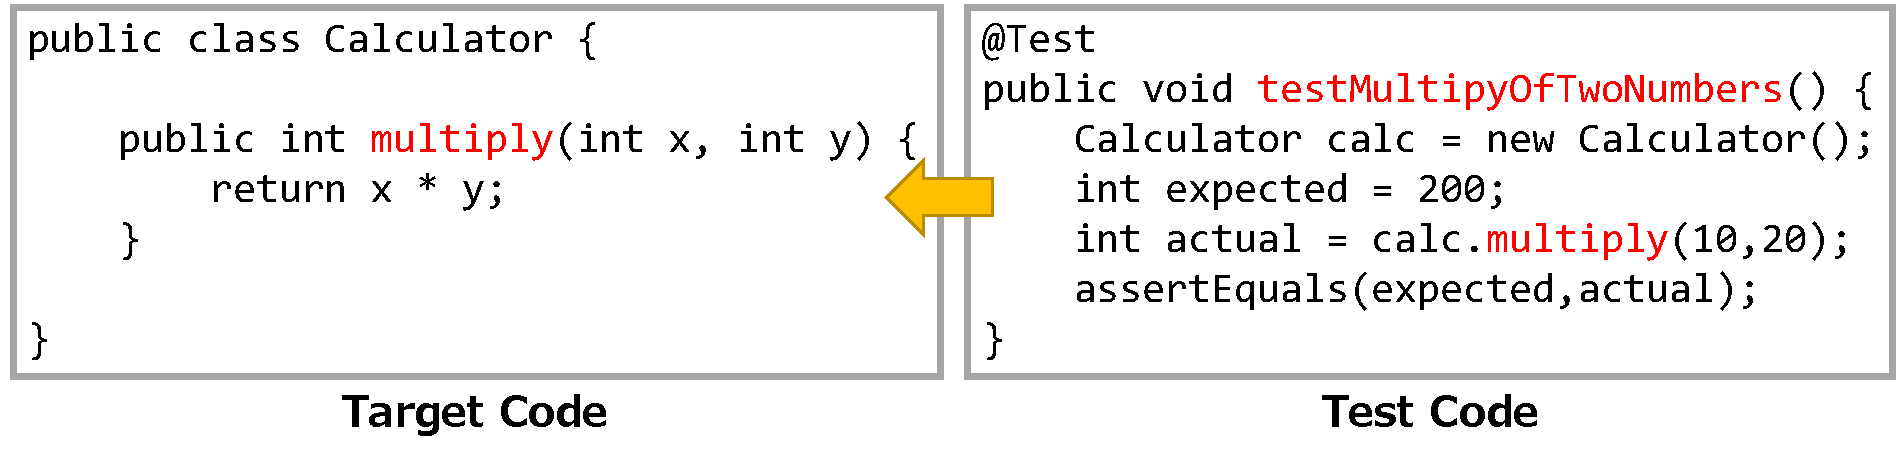
\includegraphics[width=8.5cm]{mapping.pdf}}
\caption{Example of mapping test code to target code.}
\label{fig2}
\end{figure}

\begin{enumerate}
\renewcommand{\labelenumi}{(\arabic{enumi})}
\item Statically analyze the test code and obtain the method call of the target code.
\item Divide the test method with a delimiter or capital letter and link it when the target method partially matches.
\end{enumerate}

In the unit test, the target object is generated in the test code as shown in the figure \ref{fig2}, and it is executed by calling a method of the target code. Therefore, to link the target code to the test code, the test code in the Test Code Database is statically analyzed and the method call is obtained. However, multiple methods may be called within one test method, so the method names are also compared. It is recommended to faithfully represent the contents of the processing of the target method as the test method name description method, and the name of the target method is often described in the test method name\cite{b22}. Therefore, the name of the test method is divided by a delimiter or capital letter, and it is linked if it partially matches the target method.

The Test Code Database in Figure \ref{fig1} stores test code corresponding to the production code in The Source Code Database. As a pre-processing, static analysis was performed on large-scale projects in advance, and information that linked target code and test code was stored in the DB, so that test code could be searched at high speed via the DB.

\subsection{Test Smells Detection}
In this study, tsDetect\footnote{http://testsmells.github.io/} was adopted as a test smell detection tool. tsDetect is a tool implemented with an AST-based detection method that can detect 19 test smells. It has also been reported that test smells can be detected correctly with 85\% to 100\% accuracy and 90\% to 100\% recall. In this study, We implemented to detect 6 test smells (TABLE \ref{smells}), which are important in considering the recommendation of test codes among 19 test smells that can be detected by tsDetect\cite{b9}.




\begin{comment}

\begin{table}[hbtp]
\caption{Subject Test Smells}
\begin{tabular}{|l|p{5.2cm}|}
\hline
\textbf{Name}                   & \textbf{Description}                                                                                                       \\ \hline
\textbf{Assetion Roulette}        & Occurs when a test method has multiple non-documented assertions. Multiple assertion statements in a test method without a descriptive message impacts readability/understandability/maintainability as it’s not possible to understand the reason for the failure of the test.  \\ \hline
\textbf{Conditional Test Logic} & Test methods need to be simple and execute all statements in the production method. Conditions within the test method will alter the behavior of the test and its expected output, and would lead to situations where the test fails to detect defects in the production method since test statements were not executed as a condition was not met. Furthermore, conditional code within a test method negatively impacts the ease of comprehension by developers. \\ \hline
\textbf{Default Test}            & Test code in which the test class or test method name is the default in test code using a testing framework such as JUnit. It is necessary to change the name appropriately to improve the readability of the code.                                                                                                      \\ \hline
\textbf{Eager Test }             & Occurs when a test method invokes several methods of the production object. This smell results in difficulties in test comprehension and maintenance. \\ \hline
\textbf{Exception Handling}      & This smell occurs when a test method explicitly a passing or failing of a test method is dependent on the production method throwing an exception. Developers should utilize JUnit's exception handling to automatically pass/fail the test instead of writing custom exception handling code or throwing an exception. \\ \hline
\textbf{Mystery Guest}          & Occurs when a test method utilizes external resources (e.g. files, database, etc.). Use of external resources in test methods will result in stability and performance issues. Developers should use mock objects in place of external resources. \\ \hline
\end{tabular}
\end{table}

\end{comment}

In addition, the test suites including the following four test smells that are not suitable as  have been deleted from the Test Code Database in avance, so that it is not output as a recommended test suites.

\begin{itemize}
\item \textbf{Empty Test. } It occurs when a test method does not contain executable statements.
\item \textbf{Ignored Test. } It means that test code has the @Ignore annotation and could not be executed.
\item \textbf{Redundant Assertion. } It occurs when test methods contain assertion statements that are either always true or always false. 
\item \textbf{Unknown Test. } It indicates that a test method that does not contain a single assertion statement.
\end{itemize}

\subsection{ Test Suites Recommendation}
The recommended test suites were ranked based on the similarity between the input code and the detected similar code and the number of test smells included in test suites. We investigated the relationship between the similarity between clone pairs and the similarity between test code pairs for clone pairs with test code in both code fragments on OSS projects.

As a result, there is a correlation between the similarity between the test code pairs and the similarity of the target clone pair. Therefore, we consider that the clone pairs with higher similarity between the input code and the similar code are easier to reuse the test code.

SuiteRec implements a recommendation ranking that sorts the clones in the order of high similarity and determines the order based on the number of test smells when the similarities are the same.


\begin{figure}[htbp]
\centerline{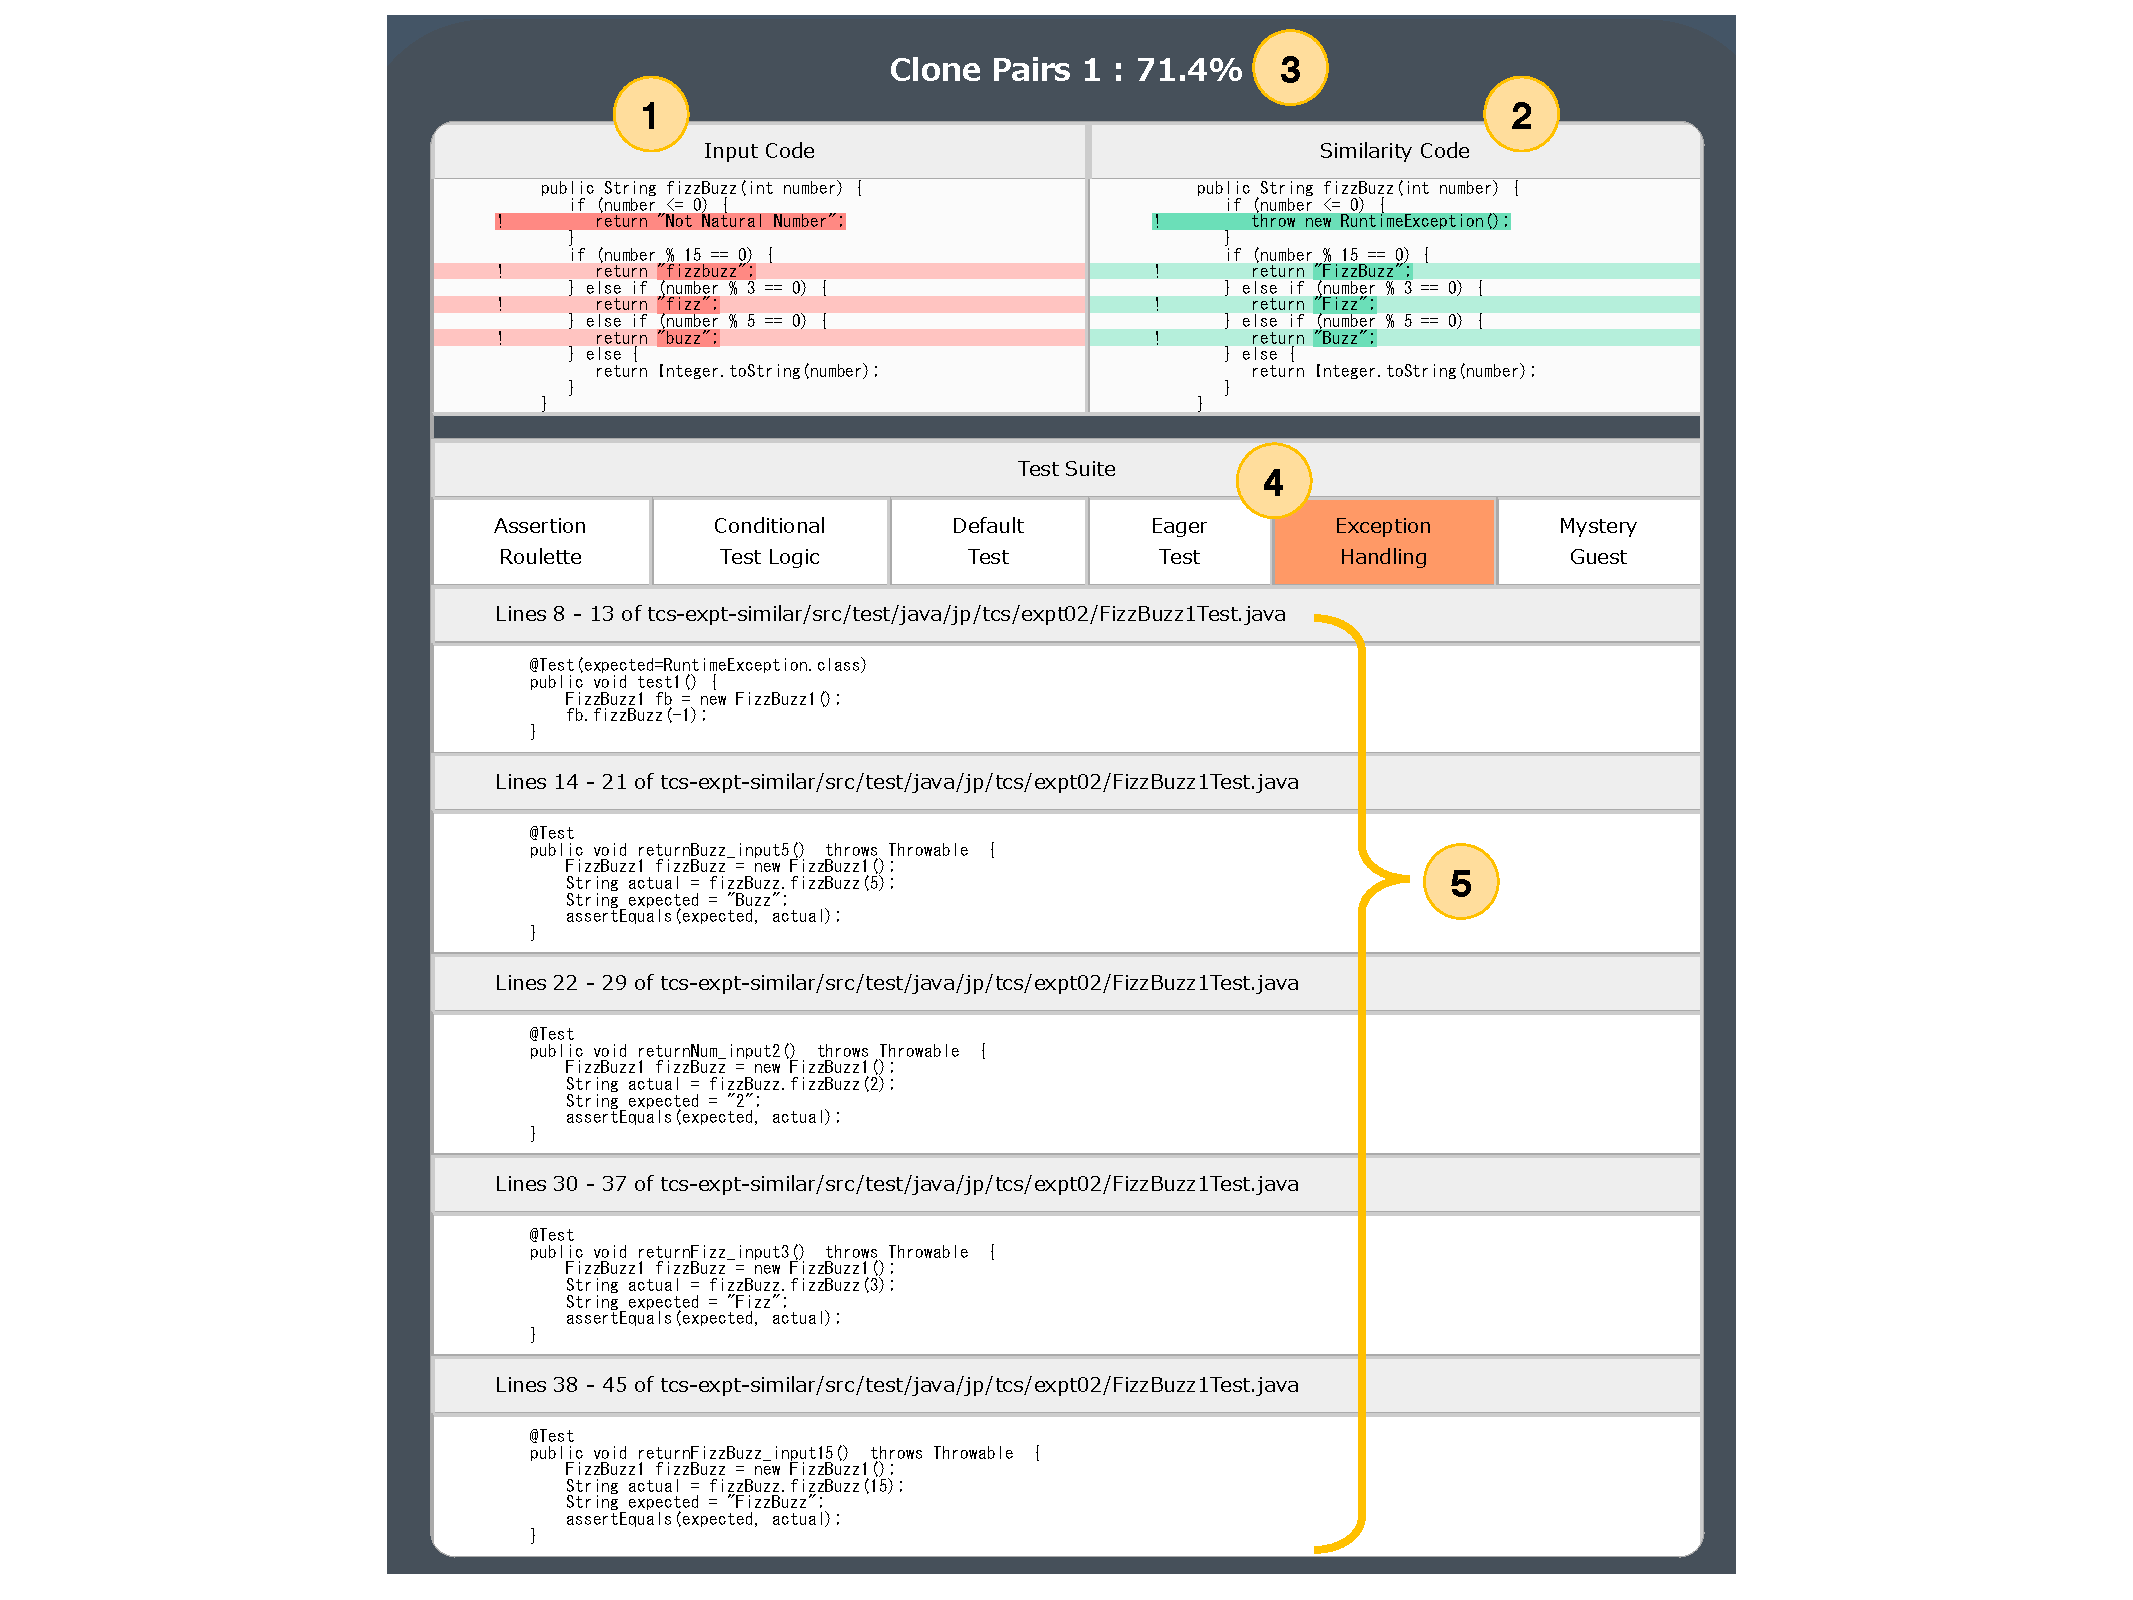
\includegraphics[width=8.7cm]{SuiteRec.pdf}}
\caption{Test suite recommended by SuiteRec.}
\label{fig}
\end{figure}

 \begin{enumerate}
\renewcommand{\labelenumi}{(\arabic{enumi})}
\item{\textbf{Input Code fragment. }The target code entered by the developer is displayed.}
\item{\textbf{Similarity Code fragment. }A similar code for the input code is displayed. The differences are highlighted so that you can see the difference between the input code and the similarity code.}
\item{\textbf{Degree of similarity. }The similarity between the input code fragment and the similar code fragment is displayed. The similarity is calculated using the Unique Percentage of Items (UPI) method used by NICAD. }
\item{\textbf{Test Smells. }If test smells are included in the test suite, test smells are highlighted in orange, and the developer is presented with the presence of test smells. }
\item{\textbf{Recommend Test Suites. }The recommended test suite is displayed. File paths are also displayed to indicate from which project the test code was referenced. }
\end{enumerate}


\section{ Preliminary User Study}
To quantitatively and qualitatively evaluate SuiteRec, we conducted a preliminary user study with 10 students developers,  aiming at answer the following four research questions:

\begin{itemize}
\item \textbf{RQ1: Can SuiteRec support the development of test codes with high test coverage?}  Test coverage is an important indicator of how well the software has been tested. We set up this RQ to confirm whether  SuiteRec can contribute to increasing  quality of the software.
\item  \textbf{RQ2: How well can SuiteRec reduce test suites  generate time?} Generally, it takes much time to generate test suites from scratch. We set up this RQ to confirm whether  SuiteRec  can  contribute to shorten the test suites generation time.
\item \textbf{RQ3: How well  SuiteRec support generate test codes with high quality?} We set up this RQ to confirm whether SuiteRec can contribute to generating high-quality test codes (i.e. with a fewer test smells).
\item \textbf{RQ4: How effective SuiteRec is to support test suites generation tasks?} We set up this RQ to confirm how well can SuiteRec support developers in generating test  suites.
\end{itemize}


%In the  preliminary user study, participants were requested to generate test suites for three different production codes. %Evaluate SuiteRec by comparing the test code with and without using SuiteRec. By collecting data on code coverage, duration of experimental tasks and test codes quality as well as qualitative survey responses, we aim to answer the following research questions:

% By collecting data on code coverage, duration of experimental tasks and test codes quality as well as qualitative survey responses, we aim to answer the following research questions:


%\subsection{Participant Selection}
%We recruited the subjects with basic programming skills and an understanding of software testing. The experiment was conducted with 10 master students who majored in information science. According to the preliminary questionnaire, more than 90\% of the subjects had more than 2 years of programming experience, and more than 80\% of the subjects had more than 1 year of Java language experience. All the subjects had basic knowledge about software testing in lectures and other situations, and more than 80\% had experience developing unit tests.
For the preliminary user study, we recruited the students who have basic programming skills and software testing knowledge. The user study was conducted with 10 master course students who majored in information science. Among participants, more than 90\% of participants had more than two years of programming experience, and more than 80\% of participants had more than one year of Java language experience. All participants had a basic knowledge about software testing with lectures  and other situations, and more than 80\% had experience in developing unit tests.


%\subsection{Object Selection}
%To conduct the experiment we prepared three production codes. It is assumed that the subjects fully understand the specifications of production code in order to develop test code. Therefore, we selected a typical computational problem that often uses competitive programming as production code. In addition, specifications written in natural language were prepared so that the specification of the production code could be confirmed. In order to make a difference in each task, the number of conditional branches in each task was increased to 8, 16, and 24.


%Figure \ref{fig4} is an example of the production code that was presented. In the post-experimental questionnaire, it was confirmed that all the subjects expressed a positive opinion about the understanding of the experimental task. Also, there was no negative answer to the question about whether there was enough experiment time. Therefore, it can be seen that the subjects fully understood the given experimental task and had sufficient work time.


% \begin{figure}[htbp]
% \centerline{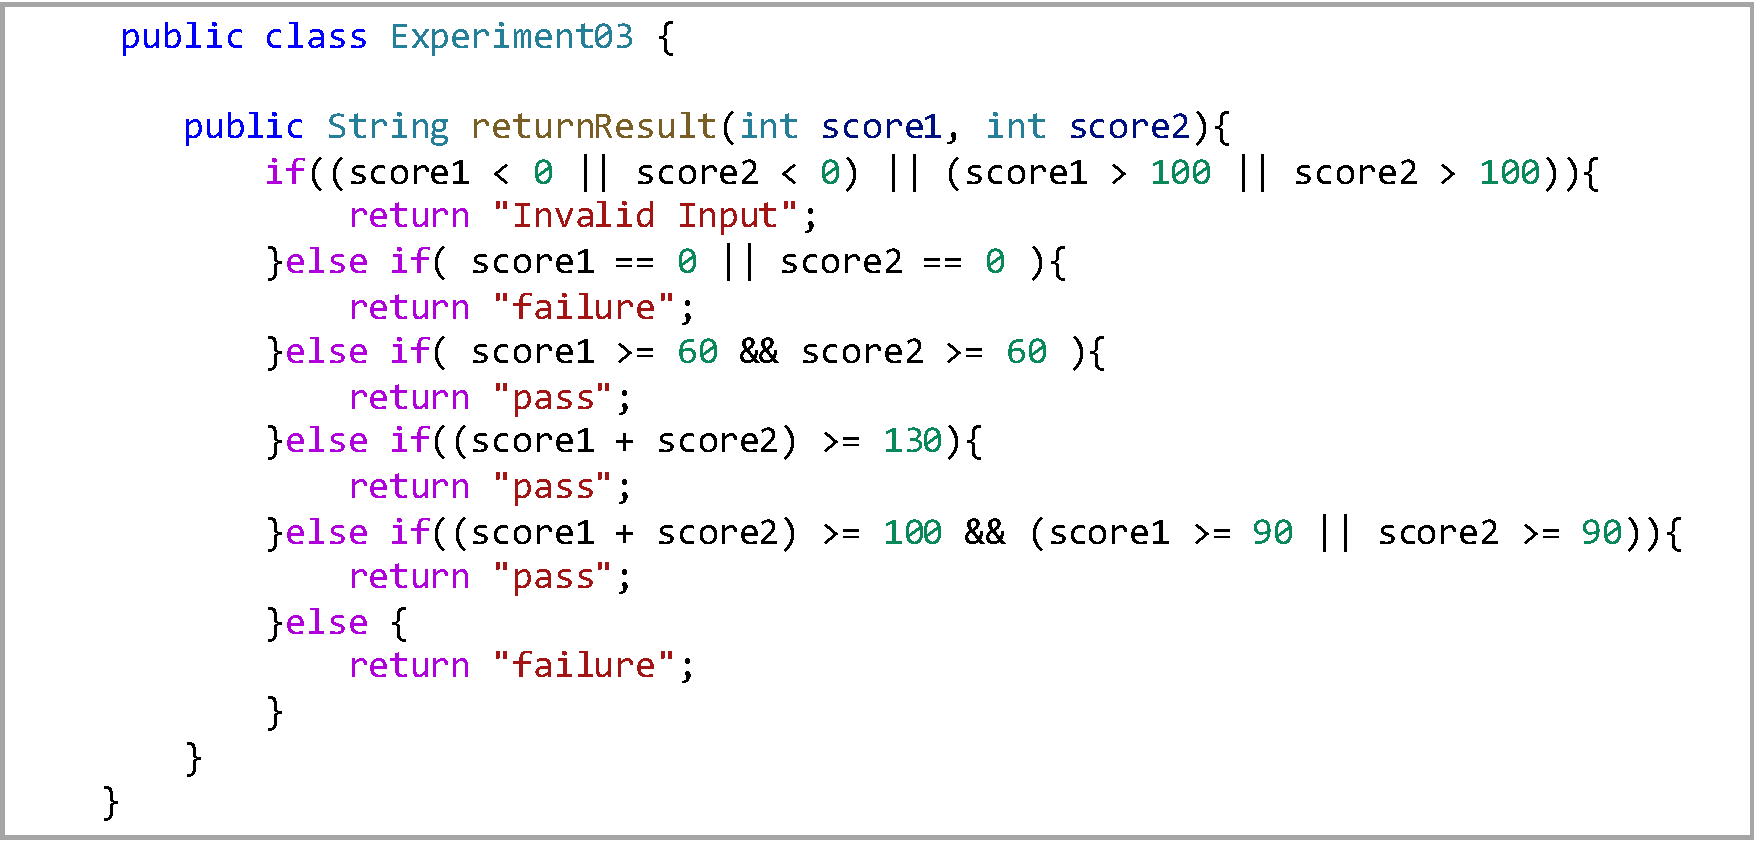
\includegraphics[width=8.5cm]{task.pdf}}
% \caption{Example of a experimental task.}
% \label{fig4}
% \end{figure}

%\subsection{Experiment Procedure}
The preliminary user study is comprised of two sessions, tutorial session and task session. 
In the tutorial session, we gave a quick lecture about basic knowledge about software testing and conducted an exercise of generating JUnit test suites to provide the deep understanding of test code generation. The tutorial session conducted during 30-minute.
%First, we conducted a 30-minute lecture and practice task on using JUnit from basic knowledge about software testing, and confirmed understanding of the test code description. And we asked them to develop test suites for the three production codes for the actual experiment.

In the task session, we assigned three tasks of creating JUnit test suites to participants with and without SuiteRec. We also requested participants to submit generated test suites. Hereafter, we call each of these assigned tasks as task1, task2 and task3.
Among assigned tasks, task 3 was relatively difficult  compared with task 1 and task 2.  In each task, we provided a production code, targets of generating test suite. The number of conditional branch in the product code used in each task was  8, 16, and 24, respectively. We also gave a requirement specification written in natural languages, so that participants could readily the understand  the specification of the production code for generating test suite.  To mitigate the learning effect of SuiteRec, participants were assigned counterbalanced tasks by dividing  into two group.  In other words, tasks were conducted with SuiteRec for task 1, without SuiteRec for task 2, with SuiteRec for task3 in the one group.  The tasks were conducted without SuiteRec for task 1, with SuiteRec for task 2, without SuiteRec for task3 for other group. Each task has a maximum of 25 minutes

The subjects were not allowed to refer to past answers. At the end, we conducted a survey to solicit feedback .

%Ask the subjects to judge the end of the experimental task. Specifically, the task was completed when the subjects were satisfied with the coverage and quality of test codes they developed. The experiment time was a maximum of 25 minutes per task.

%%%%%%%
%In the preliminary user study, we assign three tasks to generate test unites with  production codes. It is assumed that the subjects fully understand the specifications of production code in order to develop test code. Therefore, we selected a typical computational problem that often uses competitive programming as production code. In addition, specifications written in natural language were prepared so that the specification of the production code could be confirmed. In order to make a difference in each task, the number of conditional branches in each task was increased to 8, 16, and 24.
%%%%%%5
%To prevent the use effect of SuiteRec from being biased by tasks, subjects were assigned to change whether or not SuiteRec was used depending on the task. In order to prevent the learning effect when SuiteRec is used, tasks are assigned so that SuiteRec is not used continuously in three tasks. The subjects were not allowed to refer to past answers. Finally, after the completion of the experimental task, subjects were asked to answer a questionnaire on test code development.



\section{Results}
This section presents the results of quantitative and qualitative evaluation  of SuiteRec with 10 student developers, for each of the research questions.

\subsection{RQ1: Can SuiteRec support the development of test codes with high coverage?}
In this experiment, we calculated two types of code coverage: statement coverage (C0) and branch coverage (C1) of test suites submitted by the subjects. To calculate the coverage, we used EclEmma\footnote{https://www.eclemma.org/}, which is installed as a plug-in of the integrated development environment Eclipse\footnote{https://www.eclipse.org/}. Figures \ref{fig5} show the average coverage of statement coverage and branch coverage, respectively. As a result, there is almost no difference in the coverage rate of statement coverage in all three tasks depending on whether SuiteRec is used or not, and the coverage of each task exceeds 90\%.

Regarding the branch coverage in Fig. \ref{fig5}, it can be seen that there is almost no difference between TASK1 and TASK2 with 8,16 branches depending on whether SuiteRec is used or not. However, the results of TASK3 with the largest number of branches showed that there was a difference of more than 10\% in the average coverage of the subjects.

This result suggests that the test code recommended by SuiteRec is useful for increasing the coverage rate when developing test code for production code with many branches. %In fact, in the questionnaire after the experiment, there were multiple reports that the subjects were able to follow the test items that were overlooked by the recommendation code.


\begin{figure}[htbp]
\centerline{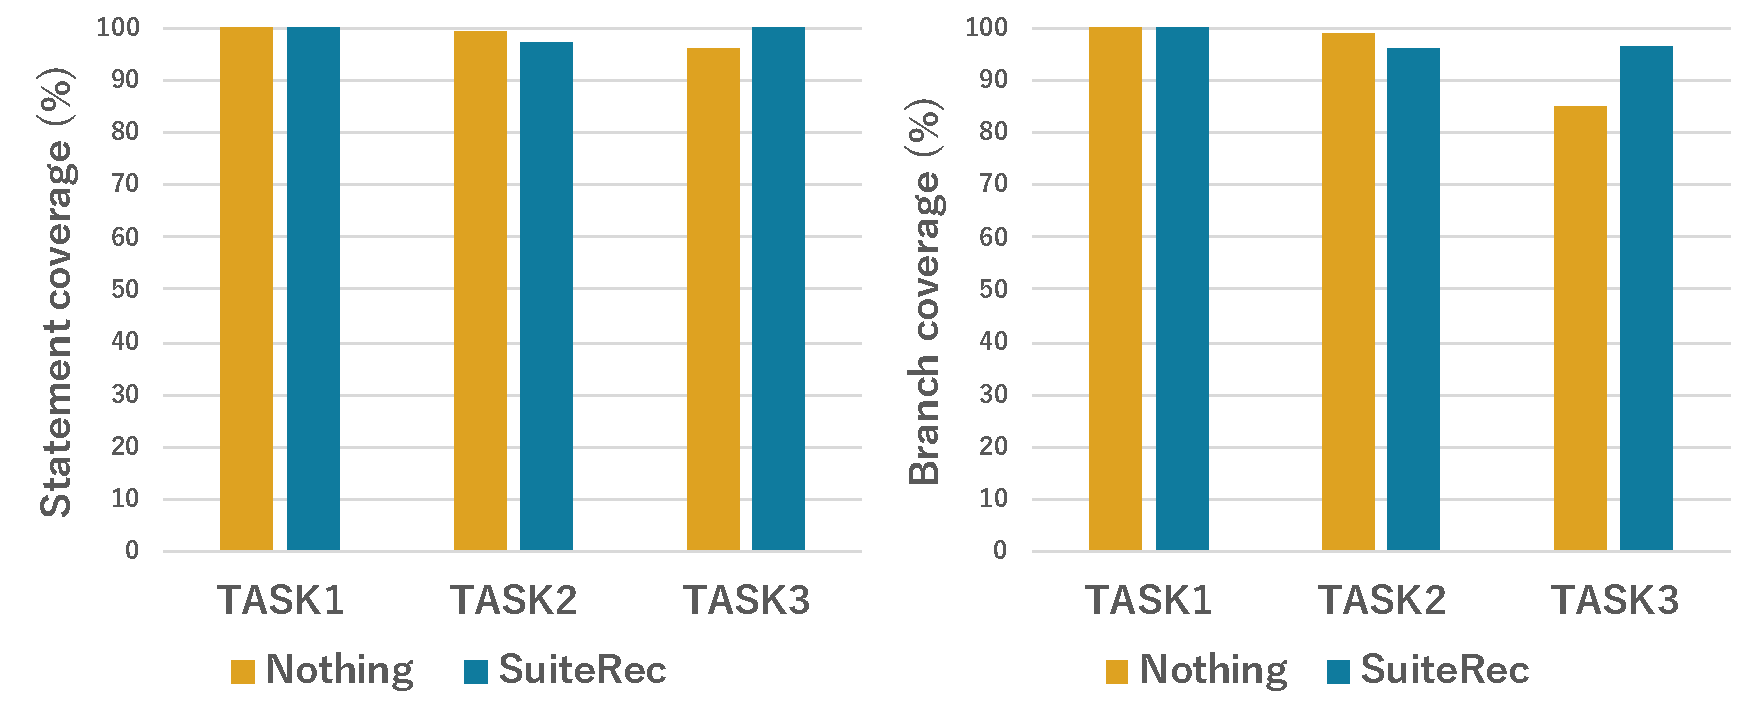
\includegraphics[width=8.5cm]{coverage.pdf}}
\caption{Code coverage (C0,C1).}
\label{fig5}
\end{figure}

% \begin{figure}[htbp]
% \centerline{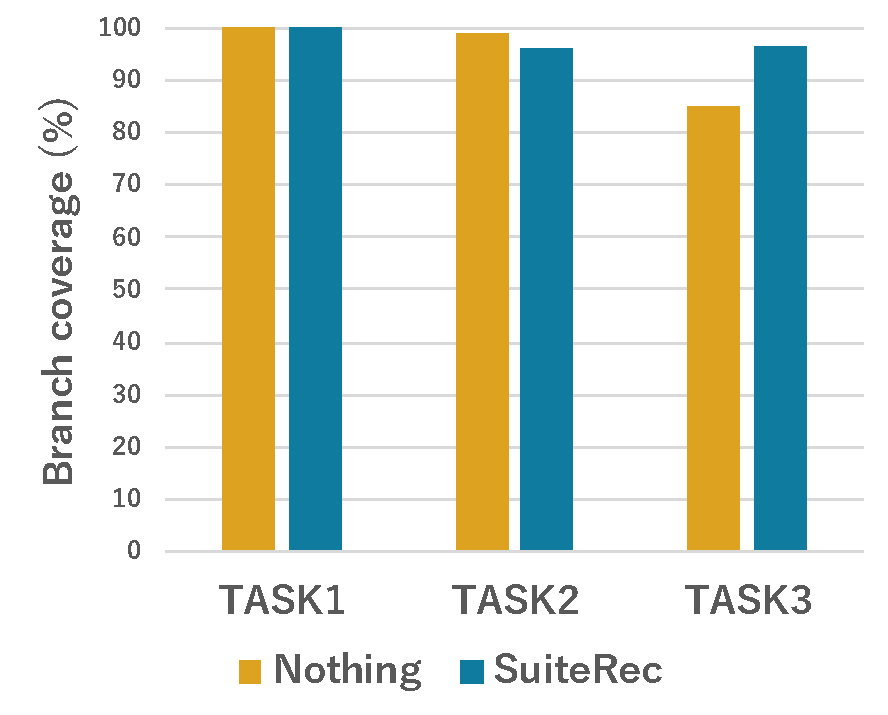
\includegraphics[width=8.5cm]{C1.pdf}}
% \caption{Branch coverage (C1).}
% \label{fig6}
% \end{figure}

\subsection{RQ2: Can SuiteRec reduce test codes development time?}
Figure \ref{fig7} shows the results of comparing the time spent completing the test code creation task with and without SuiteRec. It can be seen that the test creation time is longer when SuiteRec is used for task 1 and 3 than when it is not. This result can take time to read and understand multiple test suites recommended by SuiteRec. The subjects will not be able to reuse the recommended test codes without modification. It is necessary to edit test codes by looking at the difference between the input code and the detected similar codes. %In addition, according to the questionnaire after the experiment, it was necessary to rewrite each time the object creation statement was reused, and it took time.

For Task 2, it can be seen that the test creation time is shorter when SuiteRec is used. We investigated the submitted test codes and found that there was a lot of duplication of test cases when SuiteRec was not used even though there was no difference in coverage. This result suggests that the subjects may have wasted time developing many useless test codes.

\begin{figure}[htbp]
\centerline{\includegraphics[width=8.5cm]{duration.pdf}}
\caption{Time taken to develop test codes.}
\label{fig7}
\end{figure}

\subsection{RQ3: Can SuiteRec support the development of test codes with high quality?}
Figure \ref{fig8} shows the results of comparing the number of test smells in the submitted test suites with and without SuiteRec. For all tasks, the test codes developed using SuiteRec contains less test smell than if it were not used. This result suggests that the quality of the recommended test codes are high, and the subjects can develop the test codes while maintaining the quality by reusing them. Also, by presenting the test smells included in the recommended test suite, the test code may be rewritten based on it and a high quality test code may have been submitted. %In the actual questionnaire responses, it was reported that the test smells presented were understood and refactored to eliminate them.

%On the other hand, some subjects were aware that test smells were included, but did not know how to refactor. This is a topic for the future and needs to be improved to show how to refactor test smells.

As a whole, when SuiteRec was not used, the subjects embedded more than five times the test smells compared to the case where it was used. This is probably because many subjects did not rename the default test method and wrote the Assert statement by copy and paste within one test method. In fact, it has been reported that many of these test smells are detected in existing projects \cite{b9}.


\begin{figure}[htbp]
\centerline{\includegraphics[width=8.5cm]{smells.pdf}}
\caption{Number of detected test smells.}
\label{fig8}
\end{figure}

\begin{figure*}[t]
 \begin{center}
  \includegraphics[width=18.5cm]{qa.pdf}
  \caption{Overview of the survey responses relating to test code creation tasks}
  \label{fig9}
 \end{center}
\end{figure*}

\subsection{RQ4: How do using SuiteRec influence the developers’ perception of test code development tasks?}
% Figure \ref{fig9} summarizes answers to the survey questions. Overall, the subjects found the task clear (Question 1), and the allocated time sufficient (Question 2). For the remaining questions, you can see that there is a difference in opinion on the experimental task with and without SuiteRec. 

Figure \ref{fig9} summarizes answers to the survey questions. When developing test codes, subjects can easily feel test code creation using SuiteRec (Question 1). However, this result contrasts with the actual length of task end time (Figure \ref{fig2}), and it can be seen that the task end time is slower when SuiteRec is used. The subjects read and understand the recommended multiple test suites and determine whether to reuse them. In addition, the test code cannot be applied without modification, and it is necessary to understand the difference between the input code and the detected similar codes and make appropriate modifications to the test codes. We speculate that when using SuiteRec, subjects may spend a lot of time on this part. 

According to survey SuiteRec improvements, many responses said that it would be better to add functions that support test code editing such as a function that automatically edit classes and methods to names corresponding to the input code. Further improvements in SuiteRec show the potential for reducing the completion time of experimental tasks.

When using SuiteRec, the subjects are confident in the coverage of the test code developed by themselves (Question 2). On the other hand, 40\% of subjects reported negative responses when nothing was used. However, it is known that there is almost no difference in the coverage of the test code actually submitted (Figure \ref{fig5}). It is important to be confident in the coverage of the test codes they developed. One of the purposes of software testing is that developers are responsible for the code they develop and can provide software to users without anxiety.

When the test code was developed without using SuiteRec, 40\% of the subjects were not confident in the quality of the test code they wrote (Question 3). It can be seen that the number of test smells in the actual submitted test codes are greater when SuiteRec is not used than when it is used (Figure \ref{fig8}). Developers unknowingly embed test smells that make later maintenance activities difficult. The use of SuiteRec reduces the number of test smells and brings confidence to the code they developed by giving developers an awareness of the quality of the test code.

On the other hand, even when SuiteRec is used, there are negative opinions about the quality of the test codes. This indicates that developers who are not familiar with test smells may become confused when they were presented with test smells.
% The respondents reported that they understood Test Smells but didn't know how to refactor. This indicates the need for further improvement of SuiteRec, and we should add the function to present refactoring methods for each test smell.


\section{Related work}
{\it \textbf{Test Reuse for Clones.}} Zhang [a] et al. Proposed Grafter to transfer code between clone pairs, compare the test results before and after transplantation, and reuse the test based on that information. Soha [b] et al. Proposed Skipper that semi-automatically reuses and transforms the relevant part of the test suite corresponding to the code fragment when the developer reuses the code fragment. Skipper's approach is based on Gilligan [10], [34] and requires developers to define a detailed reuse plan to guide the conversion process. SuiteRec differs from these tools in two perspectives. First, SuiteRec searches for similar codes from projects on OSS. It is possible to find many test suites by searching in large projects. Second, SuiteRec only recommends test suites, leaving the detailed test reuse plan between clone pairs to the developer. Even if tests can be reused automatically, spreading low quality code makes maintenance difficult. SuiteRec presents test smells and gives developers confidence in the tests they developed by refactoring themselves.

\section{DISCUSSION}
\subsection{Can SuiteRec support test code development?}
When developing test codes for target codes (TASK1, TASK2) with a simple structure, it is an important result that there is no difference in coverage depending on whether SuiteRec is used (RQ1). Considering that you spend a lot of time developing test code when using SuiteRec, you can save time by developing test codes without using anything. On the other hand, when developing test codes for complex target codes with many branches (TASK3), using SuiteRec can increase the coverage by more than 10\%. This result suggests that the recommended test suite provides useful information for developers to consider test items.

Responses to the free-form questions in the survey seem to corroborate this intuition. For example, one subject stated: {\it ``I could notice test items that was overlooked by looking at the ."}

\subsection{Can SuiteRec support the development of highly maintainable test codes?}
RQ3 results showed that the quality of the test codes was high when SuiteRec was used. In the answer to free-form questions, there is a response that {\it ``I understand the presented test smells and refactored it to eliminate test smells".} Furthermore, there is a response that it was useful for improving readability, {\it ``The test method name of the  were useful when thinking about the method name".} Existing research reports that automatically generated test code is affected by test smells\cite{}. Mass generated test suites spread test smells in the project and have a significant impact on maintenance activities. this could end up being repaid during maintenance the cost that could be reduced by automatic generation. Determining whether this is the case requires further research and depends on many factors such as maintenance costs and project stability.

\subsection{Threats to Validity}
SuiteRec searches similar codes corresponding to the input code from OSS projects and recommends test suites of similar code. Therefore, the test suite cannot be recommended unless a similar code to the input code is found. Even if similar codes can be detected, if the degree of similarity is low, the recommended test suite may not be useful. NICAD detects type 2 and 3 code clones. Code clones (type 3) with insertion and deletion of statements may behave differently. In such cases, it is difficult to reuse tests. Therefore, the test suites that can be recommended may be limited to a narrow range.

\section{Conclusion and Future Work}
SuiteRec is a recommendation tool that find existing high-quality test codes from OSS projects. SuiteRec finds code clones of the input code from OSS projects and recommends test suites corresponding to the clones. The recommended test suites are sorted by their quality and presented to the developer. Furthermore, test smells, which indicate bad implementation of test codes, are shown for each test suite.

In the evaluation, we asked subjects to develop test codes with and without using SuiteRec and compared the developed test codes. We show that (1) SuiteRec improves code coverage when developing test codes for target codes with many conditional branches, (2) test codes developed using SuiteRec have higher quality and less test smells, and (3) developers feel that it is easier to develop test codes, and they are more confident in the resulting test codes when using SuiteRec.

The following tasks are planned for future work:

\begin{itemize}
\item SuiteRec needs to be improved for more practical use. Specifically, we plan to add a test code automatic editing function and refactoring function for test smells.
\item Further experiments with more subjects are needed to measure the significance of SuiteRec. In addition, To eliminate the influence of experience, it is necessary to conduct experiments not only on students but also on  engineers with extensive test development experience.
\item To investigate whether SuiteRec can be recommended in the order of preference required by developers, we plan to conduct a validity evaluation on the ranking of the test suites by subjects.
\end{itemize}



\bibliographystyle{IEEEtran}
\bibliography{reference}

%\begin{thebibliography}{15}
%\bibitem{b1} S. Shamshiri, J. M. Rojas, and J. P. Galeotti, ``How Do Automatically Generated Unit Tests Influence Software Maintenance?," In {\it Proceedings of the International Conference on Software Testing, Verification and Validation (ICST)}, pp.239--249, 2018. 

%\bibitem{b2} C. K. Roy and J. R. Cordy, ``NICAD: Accurate Detection of Near-Miss Intentional Clones Using Flexible Pretty-Printing and Code Normalization," In {\it Proceedings of the International Conference on Program Comprehension (ICPC)}, pp.172--181, 2008.

%\bibitem{b3} G. Fraser and A. Arcuri, ``EvoSuite: automatic test suite generation for object-oriented software," in  {\it Proceedings of the Symposium on the Foundations of Software Engineering (FSE)}, pp. 416--419, 2011.

%\bibitem{b4} Beck. {\it Test Driven Development: By Example.} Addison--Wesley Longman Publishing Co., Inc., Boston, MA, USA, 2002. 

%\bibitem{b4} N. Koochakzadeh and V. Garousi, ``Tecrevis: a tool for test coverage and test redundancyvisualization," Testing–Practice and Research Techniques, 2010.

%\bibitem{b5} M.Greiler, A.Zaidman, A.v.Deursen, and M.-A.Storey, ``Strategies for avoiding text fixture smells during software evolution," In {\it Proceedings of the 10th Working Conference on Mining Software Repositories (MSR)}, pp. 387--396, 2013.

%\bibitem{b6} G. Meszaros. xUnit Test Patterns: Refactoring Test Code. Addison Wesley, 2007.

%\bibitem{b7} A. van Deursen, L. Moonen, A. Bergh, and G. Kok. Refactoring test code. In {\it Proceedings of the 2nd International Conference on Extreme Programming and Flexible Processes in Software Engineering (XP)}, pp. 92--95, 2001.

%\bibitem{b8} D. Spadini, F. Palomba, A. Zaiaman, M. Bruntink, and A.Bacchelli, ``On The Relation of Test Smells to Software Code Quality," In {\it Proceedings of the International Conference on Software Maintenance and Evolution (ICSME)}, pp. 1--12, 2018. 

%\bibitem{b9} A. Peruma, K. Almalki, C. D. Newman, M. W. Mkaouer, A. Ouni, and F. Palomba, ``On the Distribution of Test Smells in Open Source Android Applications: An Exploratory Study," In {\it Proceedings of the International Conference on Computer Science and Software Engineering (CASCON)}, pp. 193--202, 2019.

%\bibitem{b10} S. U. T. Smells. http://testsmells.github.io/, 2018.

%\bibitem{b11} https://www.eclemma.org/

%\bibitem{b21} https://www.eclipse.org/

%\bibitem{b12} P. Machado and A. Sampaio, ``Automatic Test-Case Generation," Testing Techniques in Software Eng., vol. 6153, pp. 59--103, 2010. 

%\bibitem{b13} S. Panichella, A. Panichella, M. Beller, A. Zaidman, and H. C. Gall, ``The impact of test case summaries on bug fixing performance: An empirical investigation," In {\it Proceedings of the International Conference on Software Engineering (ICSE)}, pp. 547--558, 2016.

%\bibitem{b14} E. Daka, J. Campos, G. Fraser, J. Dorn, and W. Weimer, ``Modeling readability to improve unit tests," In {\it Proceedings of the Joint Meeting on Foundations of Software Engineering (ESEC/FSE)}, pp. 107--118, 2015.

%\bibitem{b15} F. Palomba, A. Panichella, A. Zaidman, R. Oliveto, and A. De Lucia, ``Automatic test case generation: what if test code quality matters?," In {\it Proceedings of the International Symposium on Software Testing and Analysis (ISSTA)}, pp. 130--141, 2016.

%\bibitem{b16} L. Ma, C. Artho, C. Zhang, H. Sato, J. Gmeiner, and R. Ramler. ``Grt: Program-analysis-guided random testing (t)," In {\it Proceedings of the International Conference on Automated Software Engineering (ASE)}, pp. 212--223, 2015.

%\bibitem{b17} A. Panichella, F. Kifetew, and P. Tonella. ``Reformulating branch coverage as a many-objective optimization problem," In {\it Proceedings of the International Conference on Software Testing, Verification and Validation (ICST)}, pp. 1--10, 2015. 

%\bibitem{b18} I. W. B. Prasetya. ``T3, a Combinator-Based Random Testing Tool for Java: Benchmarking," In {\it International Workshop on Future Internet Testing}, pp. 101--110. Springer, 2014.

%\bibitem{b19} A. Sakti, G. Pesant, and Y.-G. Gu\'{e}h\'{e}neuc. ``Instance Generator and Problem Representation to Improve Object Oriented Code Coverage," {\it Transactions on Software Engineering}, pp. 294--313, 2015.

%\bibitem{b20} M. Ellims, J. Bridges, and D. C. Ince, ``The economics of unit testing," Empir. Softw. Eng., vol. 11, no. 1, pp. 5--31, 2006.

%\bibitem{b22} F. Appel. Testing with JUnit. Packt, 2015.

%\end{thebibliography}


\begin{comment}
\vspace{12pt}
\color{red}
IEEE conference templates contain guidance text for composing and formatting conference papers. Please ensure that all template text is removed from your conference paper prior to submission to the conference. Failure to remove the template text from your paper may result in your paper not being published.
\end{comment}
\end{document}
